%!TEX root = twig-gpu.tex

\section{Method Overview}

The core idea behind our approach is to use the Twig language to represent the protocol logic of a GPU-based program in terms of types and operations on types. This has two consequences. First, by extending the existing type system, we allow a clean mixing of computational and protocol logic in our notion of located types. Second, we can leverage existing techniques from language type systems to encode operations that occur in the protocol logic. The notion of \emph{located types} that we introduce in Section~\ref{sec:located-types} is the key to our approach.

Protocol related logic is often concerned with allocation, movement, and representational conversion. Adding the concept of location to types supports a number of protocol operations, including automatic generation of allocation logic (corresponding to typed variable declaration and scoping), and device-specific representation marshalling. By extending the type system, we offload the burden of writing and optimizing this protocol logic from the programmer to automatic tools.

The advantage of pushing location information into the type system is that it forces programmers to explicitly account for operations related to the protocol logic of an application. In plain CUDA or OpenCL codes, protocol-related operations are intermixed with computational logic, and the type system does not help to enforce protocol rules. For example, in CUDA programmers are free to execute a kernel on the GPU before they have copied any data there. We will show that by augmenting type information, we can make many of these protocol-related details explicit and check them at compile time.

As we will see in Section~\ref{semantics}, programs written in Twig's language are significantly constrained with respect to control flow. The tradeoff is that Twig's constraints make it easy to reason about automated transformations on programs. In particular, we will demonstrate how the structure of Twig's language allows it to transform GPU-related programs to eliminate redundant memory copies. Other domain- or application-specific transformations will certainly be possible as well.

We illustrate the redundant memory copy problem in Figure~\ref{basic-idea}. In the figure, two GPU kernel transformations, $f$ and $g$, are combined in sequence. The top half of the diagram shows the na\"ive composition, which introduces a redundant copy. The bottom half shows the desired composition, with the redundant intermediate copies eliminated.

\begin{figure}[ht]
\begin{center}
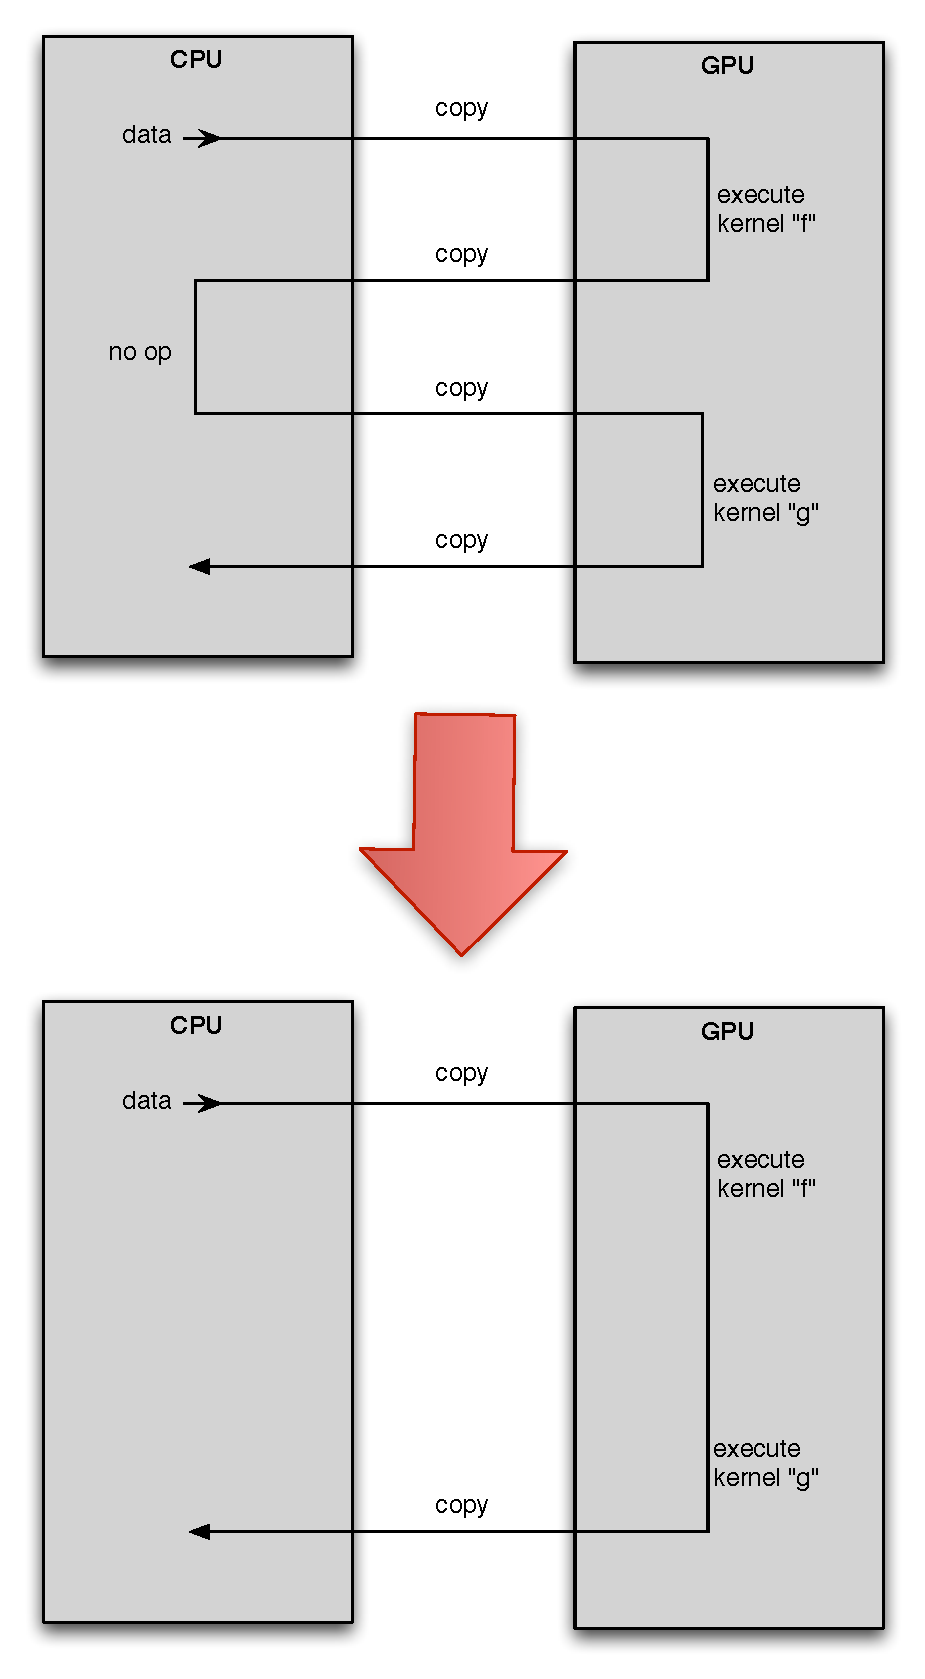
\includegraphics[width=1.8in]{images/basic-idea}
\end{center}
\caption{Elimination of redundant data copies}
\label{basic-idea}
\end{figure}

Twig operates on data types instead of data. The input to a Twig program is a data type, and the output is a transformed data type along with some generated code that will perform the transformation on data in the target language. For this reason, Twig is restricted to operate only on types that can be represented in the target language, (e.g., for C, things like \texttt{int}, \texttt{float}, or \texttt{structs}). It can, however, augment the information about those types in order to make them more restrictive. For GPU programming, we exploit this capability with the addition of \emph{located types}.

Located types are a specific instance of the notion of \emph{augmented types}, in which the types provided by a base language are enhanced to carry important semantics that are implicit in the underlying language. For example, most languages support multi-dimensional arrays, but the ordering (column versus row major) is implicit. An augmented multi-dimensional array type would add this ordering as an explicit part of the type. In this way, the transition between representations would be explicit and clear in the code, instead of something implied by the base language itself.

\subsection{Located Types}
\label{sec:located-types}

For GPU programming, we exploit Twig's augmented types by adding a notion of \emph{location} to the usual C types. Location in this case describes where the data is stored in memory, i.e., either in system memory or on the GPU.

For example, in Twig we represent an array of \texttt{int}s on the CPU as the type \texttt{array(int)}. The same type, but with the additional restriction that it be located on the GPU, is represented as \texttt{gpu(array(int))}. The general method is to \emph{wrap} an underlying type with its location. Note that the location information may or may not be reflected in the generated target type. If we are generating CUDA code, for example, the generated type for both \texttt{gpu(array(int))} and \texttt{array(int)} is simply a C pointer to \texttt{int} (i.e., \texttt{int *}). This facility allows one to express transformations in Twig which take location into account explicitly.

By wrapping the basic data type with the location information, we ensure that rules must be specific to the GPU in order to operate on GPU data. For example, a rule

\begin{verbatim}
[gpu(array(float)) -> gpu(array(int))]
\end{verbatim}

converts an ``array of floats'' data type to an ``array of integers'' type if and only if the type describes data as being located on the GPU. If the type describes data located elsewhere, it must first be converted with a rule such as

\begin{verbatim}
[array(float) -> gpu(array(float))]
\end{verbatim}

This simple but effective scheme enables automated reasoning about the movement of data across locations.

It is important to understand that rules such as those given above describe transformations on \emph{data types}, not on the data themselves. It falls to the code that is generated as a consequence of successful application of these rules to perform the promised conversion on the actual data; this is described in Section~\ref{sec:code-gen}.

While our current use of Twig's augmented type information is straightforward, our current work is focused on leveraging this capability to its fullest. Located types could, for example, be easily extended to support more complex location information. In a computer with multiple GPU devices, each device could be assigned its own location, and each location would correspond with a unique type. Furthermore, Twig may be able to use the type information in a program to infer that data should be moved between locations, and then insert the appropriate rule automatically. This process is called \emph{coercion} generation, and it is a topic of ongoing work.
